%% Solar cell makes a circuit with a 100-ohm resistor. Measure voltage
%% across resistor. Power is proportional to voltage. (Not voltage squared --
%% we must be current-limited.)
%%
%% Use PASCO Basic Optics light source. Round stand with angles
%% marked on it at the other end of the short PASCO optical bench.
%% Same setup should work tolerably well for inverse square law, or 
%% are we better off using the other light sensors there?


\section{Intensity of Solar Radiation}

\makelabheader

\bigskip
There are two main reasons winter is colder than summer:
\begin{itemize}
\item The Sun is up for fewer hours per day in the winter.
\item The Sun is lower in the sky in winter.  This means
that sunlight strikes Earth's surface at a shallow
angle, which lowers the intensity
of the radiation striking the Earth's surface.
\end{itemize}

In this lab, you'll verify these statements. In particular,
you'll find out the amount of time the Sun is up at different
times of the year,
you'll see how high the Sun rises in the sky in summer and winter,
and you'll check that radiation striking a surface at
a shallow angle deposits less energy than radiation that is
closer to perpendicular.

\bigskip

{\bf A. Amounts of sunlight at different times of the year.} 

Start up \textit{Stellarium}, and set the date to June 21, the 
first day of summer. Determine the times of sunrise and sunset on that
day, by running time forward and backward and watching the position of the Sun.
(Use a flat horizon.)
How many hours of daylight are there on that day?

\answerspace{1in}

Repeat this procedure on December 21, the first day of winter.

\answerspace{1in}

What is the ratio of these two values? That is, how many times
greater is the amount of sunlight on June 21 compared to December 21?

\answerspace{1in}

\pagebreak[2]
{\bf B. Angle made by the Sun in summer and winter.}

\medskip


Set the time to noon on June 21 (the first day of summer).
Make \textit{Stellarium} draw the \textit{meridian}, which is a line 
in the sky going from due north, directly overhead, to due south.
On any given day,
the moment the Sun crosses the meridian is the moment when it's
highest in the sky.  
At what time does the Sun cross the
meridian on this date?

\answerspace{1in}

Why doesn't the Sun cross the meridian at exactly noon?  (There
are several reasons.)

\answerspace{1.5in}

Select the Sun and view the information on it. Find the
Sun's \textit{altitude}.
This is the angle indicating the Sun's height above
the horizon. (90$^\circ$ would be directly overhead,
and 0$^\circ$ would be right on the horizon.)  What is the Sun's
maximum altitude on this date?

\answerspace{1in}

Repeat this procedure to find the Sun's maximum altitude on 
December 21, the first day of winter.

\answerspace{1in}



{\bf C. Effect of angle on the amount of solar radiation.}

\medskip

Next, you'll check to see how much of an effect this difference in angles
makes to the amount of radiation striking the Earth.  The light
bulb on your table will represent the Sun.  You will use a solar
cell to represent a small piece of the Earth's surface.
Your goal is to see how the
amount of radiation from the bulb changes as the
angle of the cell is varied. In particular, how much more radiation strikes
the cell when the light is beating down on it from almost directly above
(like sunlight in summer),
compared to the amount when the light strikes it at a shallower angle
(like sunlight in winter)?

Place the bulb at one end of the optical bench, and place
the round platform with angle markings at the other end.
We'll call the center of the round platform
the ``observer's location,'' and we'll call the bulb the ``Sun.''

Start the program called 
``solarcell.cap'' on the lab computer.  
This program allows the computer to display the amount of radiation striking
the solar cell.

Place the solar cell at the observer's location,
facing directly towards the Sun. The surface of the cell
should be perpendicular to a line going from the cell to the Sun.
In the picture below, the cell should be oriented along the
line marked ``Perpendicular.''

\centerline{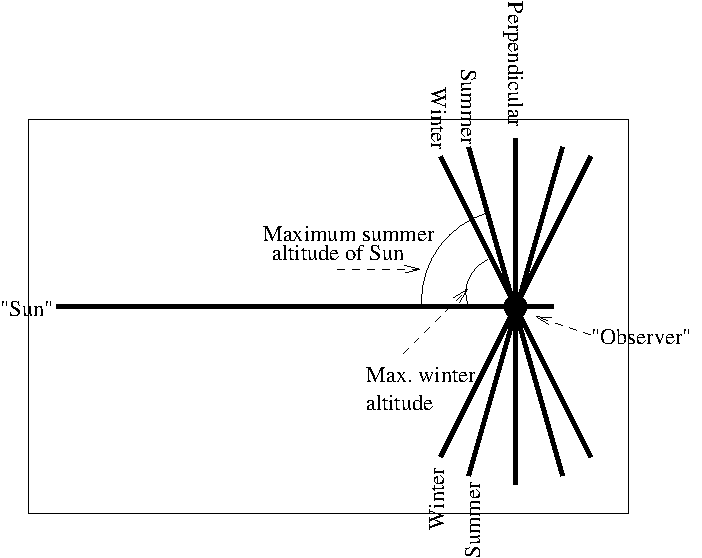
\includegraphics{solarcell/solarcellfig.pdf}}

Turn on the light bulb, and hit the ``Record''
button 
\includegraphics[width=0.2in]{solarcell/capstone-record.pdf} on the
computer screen.  You should see a graph showing the amount
of radiation striking the solar cell as time passes.  Try placing
your hand in front of the solar cell to block the light.  The
reading should go down.

Let the computer record data for about 20-30 seconds.  
We want to know the average amount of light striking the solar
cell. To find this out, you need to select a range of
data where the graph looks reasonably flat.
Hit the button that looks like this, near the top of your screen:

\includegraphics[width=0.2in]{solarcell/capstone-select.pdf}.
That'll create a rectangle that you can move to select the
region of data you want to use.
Once you've highlighted a stretch of data, the computer should
display the average (``Mean'') of those numbers.  This is the 
average amount of radiation striking the solar cell during
this time period.  Record this value:

\answerspace{0.25in}

This represents the amount of power that strikes the solar cell
if it were lying flat on the ground, and the Sun was beating down
on it from directly overhead. In fact, though, the Sun is never
directly overhead (at least, not from a location like Richmond).
The highest the Sun ever gets in the sky is the altitude you found
for the first day of summer in part B.

Rotate the solar cell so that it the angle it makes with
the line to the Sun corresponds to the altitude of the
Sun on that date. (This means orienting the cell so that it
lies along one of the lines marked ``Summer'' in the picture above.)

\pagebreak[2]

\answerspace{1in}

Repeat the procedure with the solar cell aligned on the other ``summer''
line.  

\answerspace{1in}

The last two values should be close to the same.  Average them
together:

\answerspace{1in}

Repeat this procedure with the two winter lines to end
up with an average amount of radiation striking the cell
when it's at the winter angle:

\answerspace{2in}

You should have found that the amount of radiation is greatest
when the cell is perpendicular, a bit less when it's at the summer
angle, and much less when it's at the winter angle.

How many times more intense is the midday solar radiation in summer
than in winter?

\answerspace{1in}

Let me repeat the main point. Part A and this part 
show two different reasons why it's hotter in summer: there are more
hours of daylight in summer, and the sunlight is more intense.



